\documentclass[tikz,border=30pt]{standalone}
\usepackage{amsmath,amssymb}
\usetikzlibrary{decorations.pathreplacing, calc, positioning}

\begin{document}
	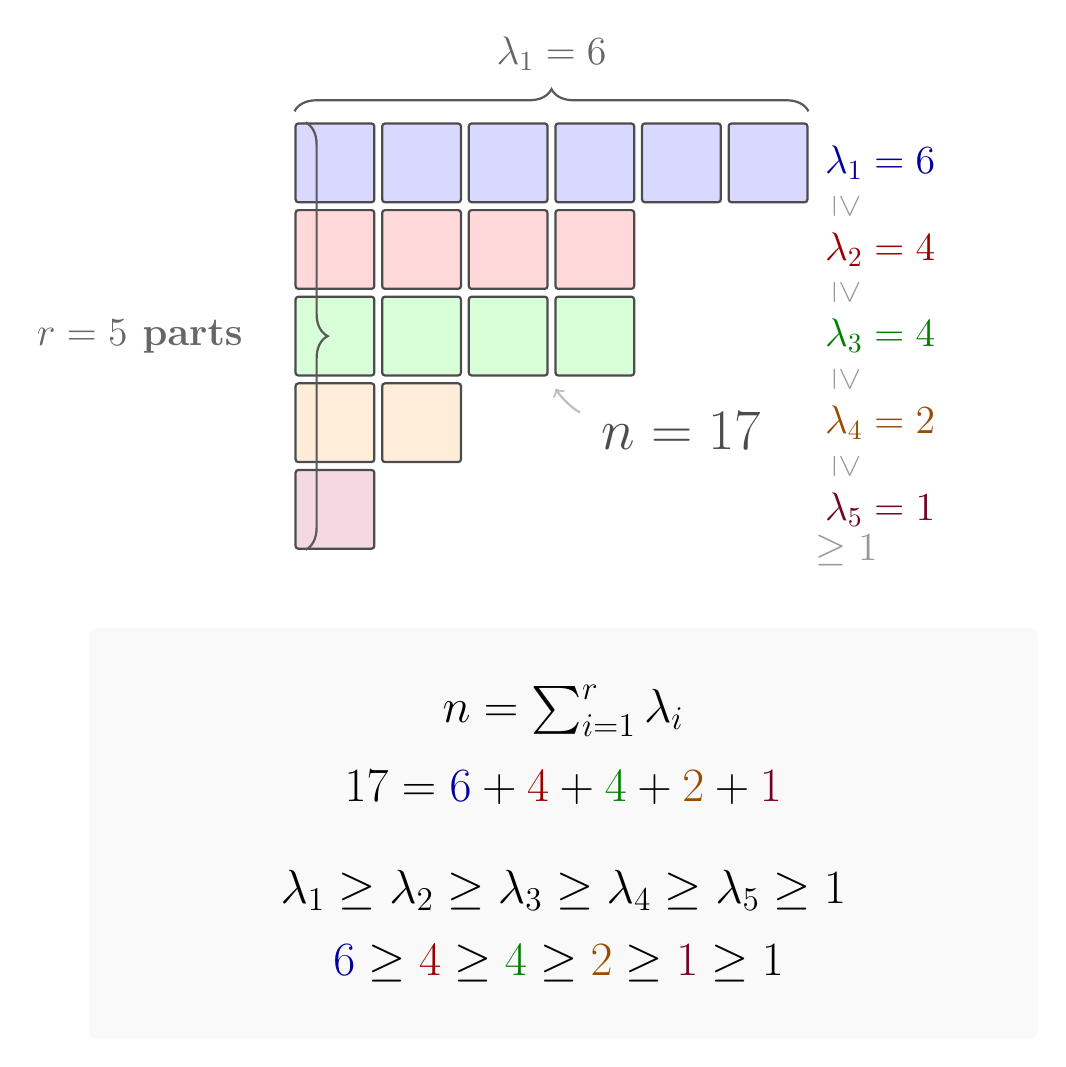
\begin{tikzpicture}[
		cell/.style={draw=black!70, thick, minimum size=1cm, inner sep=0pt, rounded corners=1pt},
		brace/.style={decorate, decoration={brace, amplitude=8pt, raise=4pt}, thick, gray!70!black}
		]
		
		% ==========================================
		% 1. DRAW THE YOUNG DIAGRAM
		% ==========================================
		% Data format: row index / length (\lambda_i) / background color / text color
		\foreach \i/\rowlen/\bgclr/\txtclr in {
			1/6/blue!15/blue!60!black,
			2/4/red!15/red!60!black,
			3/4/green!15/green!50!black,
			4/2/orange!15/orange!60!black,
			5/1/purple!15/purple!60!black%
		} {
			% Draw the sequence of blocks for the part \lambda_i
			\foreach \j in {1,...,\rowlen} {
				\node[cell, fill=\bgclr] (c-\i-\j) at (\j*1.1, -\i*1.1) {};
			}
			% Annotate the \lambda_i value on the right-hand side
			\node[anchor=west, font=\Large, text=\txtclr] (lam-\i) at (7.2, -\i*1.1) {$\lambda_{\i} = \rowlen$};
		}
		
		% ==========================================
		% 2. VERTICAL INEQUALITIES (\lambda_1 \ge \lambda_2 \dots)
		% ==========================================
		\foreach \i in {1,2,3,4} {
			\pgfmathsetmacro{\midy}{-\i*1.1 - 0.55}
			\node[font=\large, text=gray!80, rotate=-90] at (7.6, \midy) {$\ge$};
		}
		% The final \ge 1 condition
		\node[anchor=north, font=\Large, text=gray!80] at (7.6, -5.5 - 0.2) {$\ge 1$};
		
		% ==========================================
		% 3. STRUCTURAL BRACES
		% ==========================================
		% Left brace showing the total number of parts (r)
		\draw[brace, decoration={mirror}] (c-5-1.south west) -- (c-1-1.north west)
		node[midway, left=15pt, font=\Large\bfseries, text=gray!80!black] {$r = 5$ parts};
		
		% Top brace showing the largest part (\lambda_1)
		\draw[brace] (c-1-1.north west) -- (c-1-6.north east)
		node[midway, above=15pt, font=\Large\bfseries, text=gray!80!black] {$\lambda_1 = 6$};
		
		% Floating label for the total n
		\node[font=\huge\bfseries, text=black!70] (total) at (5.5, -4.5) {$n = 17$};
		\draw[->, thick, gray!50, shorten >= 5pt, shorten <= 5pt] (total) to[bend left=15] (c-3-3.south east);
		
		% ==========================================
		% 4. MATHEMATICAL TRANSLATION BOX
		% ==========================================
		\node[fill=gray!5, rounded corners=3pt, inner sep=15pt, anchor=north] (eqbox) at (4, -7) {
			\begin{minipage}{11cm}
				\centering
				\vspace{0.2cm}
				% The Summation Definition
				{\LARGE $n = \sum_{i=1}^{r} \lambda_i$} \\[4mm]
				{\LARGE $17 = \textcolor{blue!60!black}{6} + \textcolor{red!60!black}{4} + \textcolor{green!50!black}{4} + \textcolor{orange!60!black}{2} + \textcolor{purple!60!black}{1}$} \\[8mm]
				
				% The Inequality Definition
				{\LARGE $\lambda_1 \ge \lambda_2 \ge \lambda_3 \ge \lambda_4 \ge \lambda_5 \ge 1$} \\[4mm]
				{\LARGE $\textcolor{blue!60!black}{6} \ge \textcolor{red!60!black}{4} \ge \textcolor{green!50!black}{4} \ge \textcolor{orange!60!black}{2} \ge \textcolor{purple!60!black}{1} \ge 1$}
				\vspace{0.2cm}
			\end{minipage}
		};
		
	\end{tikzpicture}
\end{document}